\section{\esp Introdução}
Com a mudança de mentalidade da Web para o novo paradgma de aplicações web conhecido como Web 2.0 proposta por \cite{web20Proposta}, seus 
usuários deixaram de ter um papel passivo como consumidores de conteúdo para assumir um papel ativo de produtores de conteúdo. Esta mudança 
trouxe consigo ferramentas interativas, que tem como foco principal a geração de conteúdo por parte dos próprios usuários, tais como fóruns 
de discussões e recentemente, as redes sociais como o Twitter, Facebook e o Instagram.

Esta participação ativa dos usuários impactou significativamente a quantidade de informação disponíveis na Web. Segundo \cite{artigo01}, 
o tráfego de dados nesta rede dobra a cada ano, o que gera uma quantidade massiva de informação, tornando a Web muito influente em diversos 
setores de grande importância na sociedade, passando a fazer parte do cotidiano das pessoas que estão cada vez mais conectadas a mecanismos que
as  conectam aos conteúdos de seu interesse. Podemos perceber esta influência principalmente através das redes sociais, que segundo 
\cite{redesSociais01} estão mudando profundamente as formas de organização, identidade, conversação e mobilização social.

Como descreve \cite{deitelAjax}, com todo este conteúdo disponível, os mecanismos de busca de informação 
acabam recebendo destaque nesta ``nova Web'' e sobressaem aqueles que auxiliam os usuários  a localizar e filtrar 
as informações desejadas. Desta forma, há um grande desafio em relação à formulação de ferramentas que guie o usuário até os conteúdos de seu 
interesse, economizando assim sua atenção. Estas ferramentas com o passar do tempo se fazem mais presentes no dia-a-dia das pessoas, 
que por sua vez demandam por mecanismos cada vez mais robustos e personalizados de acordo com suas necessidades, como consequência existe 
uma demanda constante de novas aplicações mais específicas para atender determinada comunidade.

No estudo estudo realizado por \cite{perfilCicloturista}, após realizar uma pesquisa com 302 cicloturistas, concluiu-se que a internet é sem dúvidas 
o meio de informação mais utilizado por esta comunidade, totalizando 46\% das respostas em relação à qual o meio de informação utilizado por eles.
No entando, neste meio há uma demanda ainda não explorada por uma aplicação focada nesta prática, pois de acordo com \cite{cicloturismo02}, 
as grandes viagens realizadas sobre a bicicleta requerem um melhor preparo e conhecimento, por parte do ciclista, e ressalta a importância de se 
conhecer a extensão da viagem e tempo total disponível, além da região, relevo e clima escolhidos como trajeto. Devido a complexidade do planejamento
requerido, percebe-se neste meio a necessidade de uma ferramenta que centralize informações importantes para tal. Praticantes desta atividade por não 
possuírem uma ferramenta específica, recorrem a outras com propósito similares para auxiliá-los no planejamento de seus trajetos, que não oferecem 
informações importantes para este planejamento. O cicloturismo conforme descrito por \cite{cicloturismo01} é uma modalidade do ecoturismo que está 
ganhando cada vez mais adeptos no Brasil, por ser uma atividade de baixo impacto ambiental, já que é realizado com bicicletas.

Este trabalho tem como objetivo desenvolver uma ferramenta no formato rede social Web voltada a atender esta demanda de informações observada 
no meio do cicloturismo. Segundo \cite{perfilCicloturista} o  "fenômeno" cicloturismo é considerado de fraco a bom em termos de comunicação 
e estrutura para receber os cicloturistas. Com o Ciclotour, visamos prover um meio de comunicação onde usuários desta ferramenta terão acesso de 
forma centralizada a informações sobre rotas que pretendem trilhar, fornecidas por outros usuários de forma colaborativa, com o propósito 
de criar um grande repositório de informações relevantes para cicloturistas auxiliando no planejamento da atividade turística, comunicação entre 
praticantes e promoção da prática.

\section{\esp Referencial Teórico}
No princípio das aplicações Web, devido ao seu comportamento síncrono, as mesmas ficaram para trás em relação a aplicações \textit{desktop}, pois a 
interação com essas aplicações resultava em um longo período de espera conforme descreve \cite{deitelAjax}. Este atraso era causado devido à grande 
quantidade de atualizações de páginas inteiras necessárias no ciclo síncrono, demonstrado na Figura \ref{fig:arquitetura_web_tradicional}. 

\begin{figure}[!ht]
	\centering	
	\caption[\hspace{0.1cm}Aplicação Web clássica.]{Aplicação Web clássica}
	  \vspace{-0.4cm}
	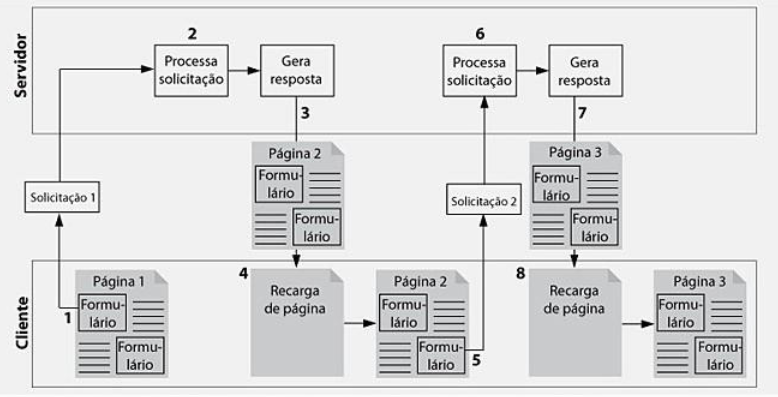
\includegraphics[width=.8\textwidth]{figuras/arquitetura_web_tradicional.png}
	 \vspace{-0.3cm}
	\\\textbf{\footnotesize Fonte: \cite{deitelAjax}}
	\label{fig:arquitetura_web_tradicional}
\end{figure}

Cada recarga na página gerava uma nova requisição ao servidor, que neste modelo é responsável por processar a requisição, gerar e enviar a resposta 
contendo a página exata que será exibida no \textit{browser} do cliente. Esse \textit{delay} presente nas interações com a aplicação fizeram com que 
os usuários ``exigissem'' uma forma melhor de interagir com estas aplicações. 

Para solucionar este problema de desempenho presente nas aplicações tradicionais, surgiu o modelo Ajax. Como descrito por \cite{garrettAjax}, uma 
aplicação Ajax elimina a natureza de interação Web conhecida como \textit{start-stop-start-stop} introduzindo uma camada intermediária 
— \textit{Ajax Engine} — entre cliente e servidor. Essa camada permitiu a essas aplicações realizarem requisições ao servidor de forma assíncrona 
e atualizar parcialmente a página ao receber a resposta, não impedindo a interação do usuário durante o ciclo de requisição/resposta. Na 
Figura \ref{fig:ajax_comparison} podemos ver um comparativo entre aplicações Web síncronas e assíncronas.

\begin{figure}[!ht]
	\centering	
	\caption[\hspace{0.1cm}Comparação aplicação Web clássica e aplicação Web com Ajax.]{Comparação aplicação Web clássica e aplicação Web com Ajax}
	  \vspace{-0.4cm}
	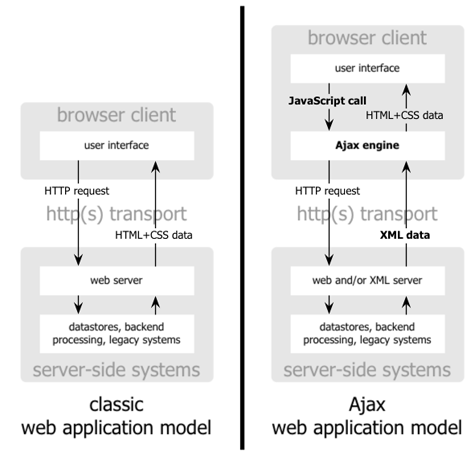
\includegraphics[width=.6\textwidth]{figuras/ajax_comparison.png}
	 \vspace{-0.3cm}
	\\\textbf{\footnotesize Fonte: \cite{garrettAjax}}
	\label{fig:ajax_comparison}
\end{figure}


Com aplicações construídas utilizando Ajax, a Web voltou à ser atrativa para usuário e tem crescido o número de aplicações Web desde então. Segundo
\cite{tabulaRest} as aplicações Web assumem atualmente uma importância sem precedentes em todas as áreas da sociedade. 

Em \cite{fieldingRest} foi apresentado o \textit{Representational State Transfer} (REST) como um estilo arquitetural para sistemas de hipermídia 
distribuídos baseado no \textit{HyperText Transfer Protocol} (HTTP). Segundo \cite{modelingRestful}, o entendimento do REST pode ajudar na obtenção 
de uma melhor performace e escalabilidade, bem como diminuir o acoplamento, como resultado aumentando a interoperabilidade, promovendo o reuso. 
Aplicações que seguem as restrições REST são denominadas como RESTful, estas aplicações consistem em um \textit{Web Service} simples que utiliza 
verbos HTTP para mapear ações as \textit{Create, Read, Update, Delete} (CRUD). Podemos ver na Tabela \ref{tab:tabela1} o mapeamento de verbos HTTP 
com as ações CRUD.

\begin{table}[htb]
	\centering
	\caption{\hspace{0.1cm} Relacionamento de verbos HTTP com ações CRUD}
	\vspace{-0.3cm} % espaço entre titulo e tabela
	\label{tab:tabela1}
	% Conteúdo da tabela
	\begin{tabular}{l|c}
  \hline
    \textbf{HTTP} & \textbf{Ação} \\
    \hline
      GET & Read \\
      POST & Create \\
      PUT & Update \\
      DELETE & Delete \\
     \hline
 \end{tabular}
 	\vspace{.1cm}  %espaço entre tabela e fonte
	\small
	% Fonte
	{\footnotesize\\ \textbf{Fonte: Elaborado pelo autor}}
\end{table}

Devido a este aprimoramento constante no que diz respeito ao desenvolvimento de aplicações Web, a arquitetura de uma aplicação Web está deixando 
de ser composta por grandes quantidades de códigos \textit{server-side}, onde todo o processamento é feito no servidor, os códigos são fechados e 
o consumo de banda é maior aos proprietários do sistema, e passando a ter maior utilização de códigos \textit{client-side}, onde o processamento dos 
\textit{scripts} da página ocorre na máquina do cliente e somente quando há necessidade de interação com o banco de dados são feitas requisições ao 
servidor \cite{spa01}. Neste contexto surgiram as \textit{Single Page Applications} (SPA) definida por \cite{spa02} aplicações composta por somente 
uma página HTML, como base para todas as outras páginas Web da aplicação nas quais as interações feitas pelo usuário são implementadas usando 
JavaScript, HTML e CSS. A Figura \ref{fig:spa} demonstra o funcionamento de uma SPA.

\begin{figure}[!ht]
	\centering	
	\caption[\hspace{0.1cm} Ciclo de vida de uma Single Page Application.]{Ciclo de vida de uma Single Page Application}
	  \vspace{-0.4cm}
	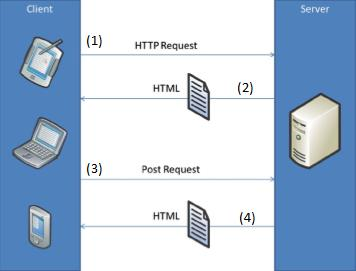
\includegraphics[width=.6\textwidth]{figuras/spa.png}
	 \vspace{-0.3cm}
	\\\textbf{\footnotesize Fonte: \cite{spa02}}
	\label{fig:spa}
\end{figure}

Em aplicações SPA, a primeira requisição realizada pelo cliente recebe como resposta uma página HTML, nesta página inicial há um extenso conteúdo de
\textit{scripts} responsáveis pela navegação do usuário, sem que haja recarga da página, quando há necessidade de conteúdos presentes no servidor, 
esta comunicação é feita através de requisições Ajax, e os scripts presentes na página são responsáveis por renderizar estes conteúdos recebidos na
página, através do \textit{Document Object Model} (DOM). Toda transição de páginas neste tipo de aplicação é realizada \textit{client-side}. 
Uma das vantagens da adoção deste modelo em relação ao modelo anterior é em relação ao \textit{overhead} de requisições, o que torna a aplicação 
mais leve e permite melhor usabilidade para o usuário final, devido ao AJAX não bloquear a manipulação da página durante sua execução \cite{spa01}, 
além de facilitar a portabilidade da aplicação pois este modelo requer uma API \textit{server-side} robusta e bem estruturada para funcionar.

\section{Trabalhos Relacionados}
\subsection{Runtastic}
A rede Runtastic \cite{runtastic}, reúne várias modalidades de esportes como ciclismo, corrida ou triatletismo. Oferece a seus usuários a
possibilidade de registrar suas atividades e performace obtida, com propósito de montar estatísticas que podem ser compartilhadas com seus amigos e
usadas para medir seu progresso. Esta rede social está associada a várias práticas físicas, com seu foco voltado ao treinamento. É munida de 
estatísticas para auxiliar em análises de desempenho de atletas em geral e não somente ciclistas. Suas rotas tem como finalidade demarcar o trajeto 
e progressos físicos em rotinas de treinos. As funções desta rede não abrangem atividades turísticas. Esta rede possui o recurso de enviar fotos de 
momentos durante sessões de atividades físicas realizadas pelo usuário. A rede  possui duas opções de idiomas inglês e alemão. Permite utilizar 
aplicativo \textit{mobile} para acompanhamento e GPS para gerar as estatísticas com base na atividade realizada. Como recursos de rede social, o 
Runtastic permite relacionamento de amizade entre usuários, \textit{posts} no mural de outros usuários, acompanhamento em tempo real através de um 
mapa a  atividade realizada por outros usuários, enviar \textit{cheers} para o usuário que está realizando a atividade, além de permitir curtir e 
comentar a atividade realizada. 

\subsection{Strava}
A rede Strava \cite{strava} possui diversas funções voltadas à prática de atividades físicas diárias, focadas em caminhadas/corridas e ciclismo. Esta
rede possibilita seus usuários ao redor do mundo registrarem seus esforços físicos diariamente, pois possui um registro de atividades físicas visando 
comparar o seu progresso. Oferece a seus usuários desafios para estimulá-los a aumentar sua performance, possui o recurso de traçar rotas com o 
objetivo de planejar a atividade esportiva e treinamento. Nesta rede é possível cadastrar metas personalizadas relacionadas a desempenho, 
possibilitando seus usuários um acompanhamento de seu progresso em suas atividades, além possuir quadros informativos sobre distâncias percorridas 
em relação a espaços de tempo. Como recursos de rede social, o Strava permite ao usuário seguir outros usuários, ingressar em grupos de usuários 
denominados clubes que podem ser públicos ou privados, possui um \textit{feed} de atividades onde são exibidas atividades realizadas por todos os 
usuários da rede, neste \textit{feed} são exibidas fotos compartilhadas durante a realização destas atividades e a rota percorrida com informações 
de distância total e horário inicial e final da atividade. Esta rede possui um aplicativo \textit{mobile} que registra através do uso do GPS a 
atividade do usuário e permite ao mesmo compartilhar fotos tiradas durante o percurso. O Strava não oferece nenhum recurso voltado a atividades 
turísticas.

No Quadro 1 podemos ver um quadro comparativo entre as funções do Ciclotour e das redes analisadas.

   \begin{center}
          \centering
       	\textbf{Quadro 1 - Comparação entre funcionalidades das Redes e o Ciclotour}\\
        \label{quadro1}
	\begin{tabular}{|c|c|c|c|} \hline
	\multicolumn{4}{|c|}{\textbf{Comparação entre funcionalidades das Redes e o Ciclotour }} 	  \\
		\hline \textbf{ Funções } & Strava & Runtastic & Ciclotour \\  
		\hline \textbf{ Criar rotas personalizadas } & SIM & SIM & SIM \\ 
		\hline \textbf{ Criar pontos informativos em rotas } & NÃO & NÃO & SIM  \\
		\hline \textbf{ Indicar tipo do terreno da rota } & SIM & SIM & SIM \\ 
		\hline \textbf{	Adicionar Fotos à Rota } & NAO & NAO & SIM \\ 
		\hline \textbf{ Comentários em rotas }	& NÃO & SIM & SIM \\ 
		\hline \textbf{	Comentários em pontos } & NAO & NAO & SIM \\ 
		\hline \textbf{	Marcar rotas como realizadas ou pendentes } & NAO & NAO & SIM \\ 
		\hline \textbf{	Permitir relação de amizade entre usuários } & NÃO & SIM & SIM \\ 
		\hline \textbf{	Buscar rotas com base em origem e destino } & NÃO & NÃO & SIM \\ 
		\hline
	\end{tabular}
	\vspace{0.1cm} 
	{\footnotesize\\ \textbf{Fonte: Elaborado pelo autor}}
   \end{center}

\section{Metodologia}
O ciclo de desenvolvimento da aplicação Ciclotour foi dividido nas seguintes fases: Coleta inicial de requisitos, teste de aceitação via 
\textit{mockup} por parte do fornecedor de requisitos, implementação das \textit{features} aceitas e teste final de aceitação. Para isso 
o desenvolvimento do Ciclotour contou com uma abordagem \textit{top-down}. Nesta abordagem o \textit{front-end} é construído antes do 
\textit{back-end}. Foi adotada esta abordagem de desenvolvimento pois desta forma é possível aprovar o funcionamento do sistema a partir de um 
\textit{mockup} de como seria a usabilidade de cada tela do sistema, sem necessidade de implementar toda a aplicação. Assim, o ``custo'' de mudanças 
é reduzido, pois além do que foi contruído ter passado por uma pré-aprovação do fornecedor de requisitos, o maior custo de mudanças se dá em 
alterações de modelos de banco de dados, que só será implementado após aprovação, evitando que sejam necessárias este tipo de mudança. Desta forma é 
possível evitar retrabalho. Nos próximos parágrafos serão descritas as fases do ciclo de desenvolvimento da aplicação Ciclotour.

Na fase de coleta inicial de requisitos, foi realizada uma reunião com cicloturistas que são os principais fornecedores de requisitos para a 
aplicação. Nesta fase, foram expostos os principais problemas enfrentados pelos fornecedores durante o planejamento de sua atividade, as 
ferramentas que eram utilizadas para auxiliar na solução destes problemas, além de informações que os fornecedores de requisitos tinham maior
dificuldade de encontrar. Após esta reunião, foram executadas análises destes requisitos e gerada uma proposta inicial de solução que foi apresentada
ao envolvidos. Após a aprovação desta proposta, iniciou-se a contrução do \textit{mockup} que será utilizado na próxima fase.

Após finalizar a construção do \textit{mockup} onde é possível interagir de forma prototipada com o sistema, percebendo o funcionamento das 
\textit{features} envolvidas, usabilidade e o \textit{workflow} de como será o sistema, é realizado um teste de aceitação por parte dos 
cicloturistas envolvidos no projeto para antecipar o \textit{feedback} em relação às mudanças necessárias, com o objetivo de adequar a aplicação às 
espectaticas do usuário. Esta fase foi executadas em várias iterações, até que o \textit{mockup} fosse totalmente aprovado pelos fornecedores de 
requisitos e só então começar a construção do \textit{backend}.

Tendo um protótipo aprovado, iniciou-se a fase de implementação das \textit{features} do Ciclotour. Nesta fase, foi utilizada a técnica conhecida 
como \textit{Test Driven Development} (TDD). Esta técnica tem como princípio o desenvolvimento guiado por testes, visando garantir que o que foi 
desenvolvido está correto, evitando assim retrabalho. Utilizando esta técnica é possível garantir a conformidade com requisitos e prevenção de 
\textit{bugs} que possam surgir. 

Cada \textit{feature} implementada gerou um \textit{deploy} da aplicação para o servidor, onde foi possível que os fornecedores de requisitos testassem
e retornassem um \textit{feedback} o quanto antes, evitando maiores impactos por conta de mudanças necessárias. Essa fase junto à fase de 
implementação ocorreu de forma interativa, até que o sistema estivesse totalmente construído.

Este ciclo de desenvolvimento foi escolhido para o desenvolvimento da aplicação Ciclotour pois desta forma foi possível minimizar o retrabalho ao 
máximo, o que no caso deste trabalho era de extrema importância devido ao curto período de tempo disponível para realiza-lo. 

\section{\esp Ferramentas}

\subsection{Servidor}
Para desenvolver o \textit{server-side} da aplicação Ciclotour, foram utilizados o \textit{framework} Python de desenvolvimento Web Django com a 
extensão Django REST Framework para construção de \textit{Web Services}. O Django utiliza um estilo arquitetural baseado no 
\textit{Model-View-Controller} (MVC), o \textit{Model-View-Template} (MVT). Na aplicação Ciclotour, o Django é responsável por processar a 
solicitação inicial onde a página contendo todos os \textit{scripts} necessários para a aplicação é devolvida como resposta para o solicitante,
manter uma interface de administração do sistema e manter os modelos do sistema através de seu \textit{Object-relational mapping} (ORM). 
As requisições posteriores enviadas ao servidor serão requisições de dados que serão processadas e respondidas pelo Django REST \textit{framework} 
em formato \textit{JavaScript Object Notation} (JSON).

\subsection{Cliente}
Para desenvolver o \textit{client-side} da aplicação Ciclotour foram utilizados o \textit{framework} JavaScript AngularJS e o \textit{framework} 
CSS Bootsrap, além da API JavaScript do GoogleMaps. O AngularJS tem como propósito permitir a construção de elementos \textit{client-side} de forma 
declarativa, através de suas diretivas. Este \textit{framework} também adota o estilo arquitetural MVC, além de prover uma abstração para as chamadas
Ajax e atualização em tempo real do \textit{Document Object Model} (DOM) através do \textit{Two-way Data Binding}, o que promove uma melhor 
organização do projeto que por se tratar de uma SPA, possui alto grau de complexidade em seus scripts. Devido a esta facilidade oferecida pelo 
\textit{framework}, o AngularJS foi utilizado desenvolver de todos os scripts \textit{client-side} da aplicação Ciclotour. O Bootstrap foi utilizado 
com o intuito de oferecer uma interface rica e com \textit{design} responsivo para promover melhor usabilidade e experiência por parte do usuário 
final do sistema. Para prover recursos geográficos que possibilitem interação do usuário de forma intuitiva, a aplicação Ciclotour conta com a API 
Javascript de mapas do Google, o GoogleMaps, que oferece recursos gráficos para renderização de mapas interativos, além de recursos para obter menor 
distância entre pontos e diversos recursos geográficos.

\section{Aplicação Ciclotour}
O Ciclotour foi desenvolvido com o principal objetivo de atender às demandas específicas percebidas no meio do cicloturismo, uma atividade que exige
um extenso planejamento por parte do praticante e que carece de meios de informações focados em suas atividades. Os requisitos para esta aplicação
são: A aplicação deve ser construída em formato rede social 100\% focada em cicloturismo, com o propósito de centralizar informações sobre 
cicloturismo. Nesta aplicação deve ser possível cadastrar rotas personalizadas, de forma que os próprios usuários alimentarem a base de dados com 
o trajeto, os lugares para dormir, para comer, pontos turísticos interessantes, lugares que não valem a pena passar e etc. Deve ser possível que 
usuários expressem suas opiniões e façam observações e envie fotos sobre estas rotas e lugares.

Para tal, o Ciclotour foi desenvolvido adotando uma arquitetura centrada em dados, de forma a se tornar um grande repositório de informações 
específicas ao meio do cicloturismo aliementado pelos próprios usuários de forma colaborativa. Assim, será possível centralizar informações que 
estão disponíveis de forma esparsa na Web em um único local e auxiliar os cicloturistas em seu planejamento sem que o mesmo precise extender sua 
pesquisa às infinitas fontes espalhadas por toda internet. Para alcançar este objetivo, o Ciclotour foi desenvolvido no formato de rede social, para 
estimular o compartilhamento de informações por parte de seus usuários, através de interações por comentários, cadastro de rotas personalizadas, 
cadastro de pontos em rotas e envio de fotos para rotas. Nas seções seguintes serão detalhadas todas as funcionalidades da aplicação.

Para o desenvolvimento do Ciclotour, foi utilizado o estilo arquitetural RESTful, sendo este sistema contruído como uma SPA. Desta forma, há
uma separação completa das responsabilidades entre cliente e servidor, onde a responsabilidade de composição das páginas é delegada ao 
\textit{browser} executado \textit{client-side} e o servidor passa a atuar apenas como um repositório dos dados pertinentes à aplicação. A Figura 
\ref{fig:estruturaCiclotour} demonstra a estrutura simplificada entre cliente e servidor da aplicação Ciclotour, e as tecnologias utilizadas para
a construção do sistema.

\begin{figure}[!ht]
	\centering	
	\caption[\hspace{0.1cm} Estrutura simplificada entre cliente e servidor da aplicação Ciclotour.]
	{Estrutura simplificada entre cliente e servidor da aplicação Ciclotour}
	  \vspace{-0.4cm}
	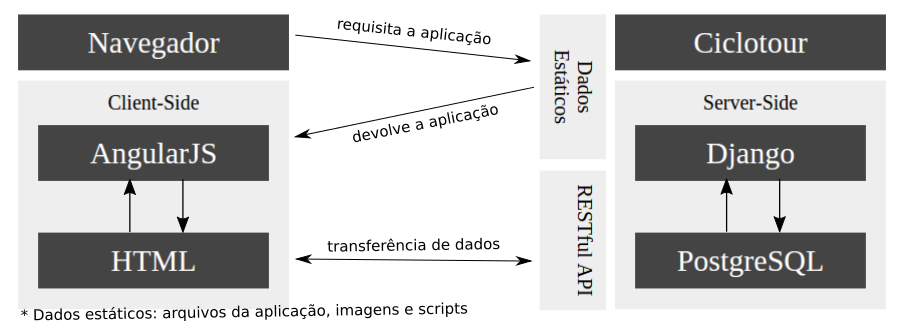
\includegraphics[width=1\textwidth]{figuras/estruturaCiclotour.png}
	 \vspace{-0.3cm}
	\\\textbf{\footnotesize Fonte: Elaborado pelo autor}
	\label{fig:estruturaCiclotour}
\end{figure}

\subsection{Cadastro de rotas}
A aplicação Ciclotour conta com uma funcionalidade de cadastro de rotas personalizadas, possibilitando ao usuário traçar rotas de forma interativa 
através de simples cliques em um mapa. Para tal, basta que o usuário informe uma origem e após preencher este campo, será exibido um mapa na 
tela da aplicação centralizado na origem informada pelo usuário. Para continuar o cadastro da rota, basta que o usuário clique no mapa marcando os 
pontos para traçar a rota conforme demonstrado na Figura \ref{fig:cadastroRotas}. O Ciclotour conta com duas formas de traçar a rota entre estes 
pontos, sendo a forma automática, que permite ao usuário traçar a melhor rota que interliga estes pontos, fornecida pela API do GoogleMaps ou a 
forma manual, em que a rota entre os pontos será uma linha reta. Além destas informações, o usuário deve fornecer um título para esta rota, uma 
descrição, e a informação do tipo de terreno desta rota. 

Feito isto, o usuário tem a possibilidade de restringir o acesso desta rota, visando garantir sua privacidade. As opções disponíveis para privacidade de 
rotas são: privada, pública e restrita aos amigos. Na opção privada, somente o usuário terá acesso à esta rota, enquanto na opção pública todos os 
usuários do Ciclotour poderão interagir com a rota. Além destas opções, o Ciclotour ainda permite ao usuário configurar a rota como restrita à amigos, 
de forma que somente os amigos do usuário que criou a rota poderão interagir com a mesma. Os tipos de terreno disponíveis inicialmente no sistema 
são: montanhoso, estrada, estrada de terra, trilha e praia. Novos tipos de terreno podem ser cadastrado na interface de administração do sistema 
conforme for necessário.

\begin{figure}[!ht]
	\centering	
	\caption[\hspace{0.1cm} Cadastro de Rotas da aplicação Ciclotour.]
	{Formulário de cadastro de rotas da aplicação Ciclotour}
	  \vspace{-0.4cm}
	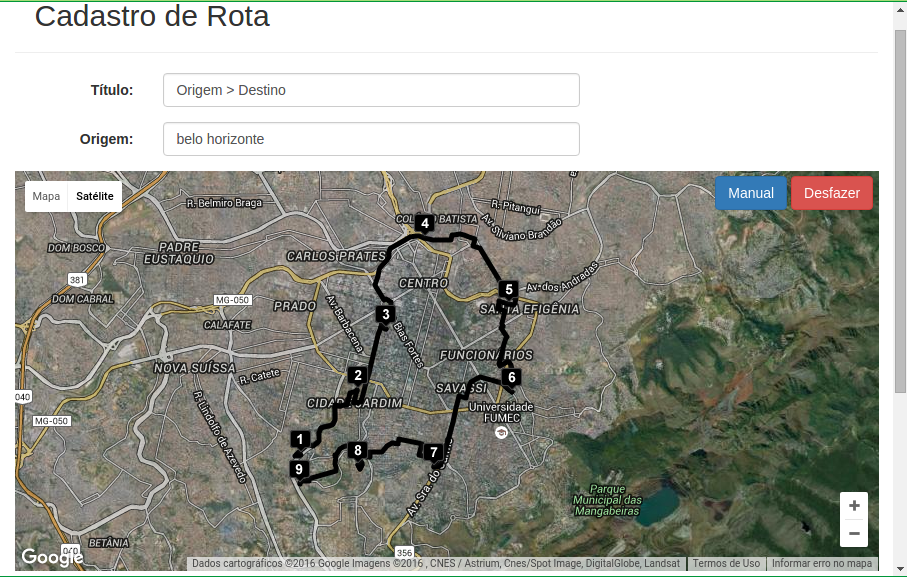
\includegraphics[width=0.8\textwidth]{figuras/cadastroRotas.png}
	 \vspace{0cm}
	\\\textbf{\footnotesize Fonte: Elaborado pelo autor}
	\label{fig:cadastroRotas}
\end{figure}

\subsection{Cadastro de pontos em rotas}
Uma informação muito importante para cicloturistas é o que poderão encontrar durante seu percurso nas rotas. É de extrema importância para um 
cicloturista saber por exemplo, onde ele pode encontrar pontos de paradas como restaurantes, pousadas, hotéis, pois muitas vezes as rotas percorridas
por estas pessoas é extensa e podem inclusive durar dias. Para isto, a aplicação Ciclotour possui um cadastro de pontos informativos em rotas, onde
usuários podem cadastrar pontos em determinada rota, bastando clicar sobre ele no mapa da rota e informando um título, o tipo do ponto e uma 
descrição. O sistema irá gerar automaticamente o endereço do ponto, conforme visto na Figura \ref{fig:cadastroPonto}. 

O sistema inicialmente conta com 6 tipos de pontos, sendo eles: Natureza exuberante, pontos turísticos, estadia, restaurante, alerta e proibição. 
Cada tipo possui um ícone que será exibido no mapa, facilitando ao usuário a identificação. Na interface de admnistração do sistema é possível 
cadastrar novos tipos de pontos, conforme for necessário. Estes tipos de ponto iniciais do sistema foram levantados com o fornecedor de requisitos 
como sendo os principais pontos de interesse para cicloturistas em uma rota.

\begin{figure}[!ht]
	\centering	
	\caption[\hspace{0.1cm} Cadastro de Pontos em Rotas da aplicação Ciclotour.]
	{Formulário de cadastro de ponto em uma rota da aplicação Ciclotour}
	  \vspace{-0.4cm}
	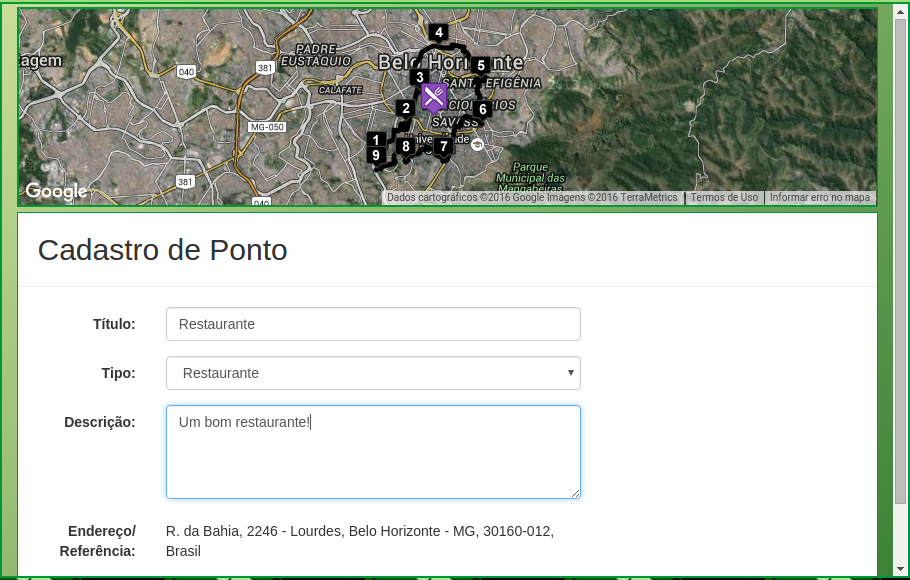
\includegraphics[width=0.8\textwidth]{figuras/cadastroPonto.png}
	 \vspace{0cm}
	\\\textbf{\footnotesize Fonte: Elaborado pelo autor}
	\label{fig:cadastroPonto}
\end{figure}

\subsection{Comentários em Pontos e Rotas}
Fóruns na Web geram uma grande quantidade de informações a partir da interação entre usuários. Pensando nisto, a aplicação Ciclotour conta com uma 
sessão de comentários em Rotas e em Pontos, possibilitando o interação entre usuários e permitindo ao usuário expor suas observações e ponto de 
vista, desta forma gerando informações relativas a estes pontos e rotas que podem ser aproveitadas por outros usuários, além de ser um local onde 
usuários podem tirar dúvidas com outros usuários que já realizaram tal rota ou passaram em tal ponto.

\subsection{Buscar rotas}
Ao entrar na página de buscas de rotas, serão exibidas as rotas cadastradas ordenadas por sua data de cadastro, exibindo as mais recentes.
O Ciclotour possui a opção busca por rotas a partir de origem e destino, onde o usuário pode informar de onde deseja partir e até onde deseja chegar,
e o sistema irá retornar as rotas já cadastradas que atendam à esta condição. Para esta funcionalidade, foi utilizado um raio de 5 km entre as 
coordenadas do ponto de origem e destino informados pelo usuário. Ao informar origem e destino, o sistema automaticamente converte o texto em 
coordenadas utilizando a API do GoogleMaps, e realiza um cálculo de raio de 5 km e busca as rotas cadastradas que possuem seu primeiro e último ponto
dentro do raio de 5km da origem e destino informadas pelo usuário respectivamente.

\subsection{Marcar rotas como realizadas ou pendentes}
A aplicação Ciclotour permite ao usuário marcar as rotas como realizadas ou pendentes conforme a Figura \ref{fig:marcarRota}, possibilitando que o 
mesmo organize suas próximas atividades através das rotas pendentes, as quais o usuário deseja realizar. Além de poder marcar rotas como pendentes, 
o usuário poderá marcá-las como realizada e a quantidade de rotas pendentes e realizadas pelo usuário serão exibidas para os outros usuários do 
Ciclotour.

\begin{figure}[!ht]
	\centering	
	\caption[\hspace{0.1cm} Marcar rotas como realizadas ou pendentes.]
	{Página de visualização da Rota onde é possível o usuário marcá-la como realizada ou pendente}
	  \vspace{-0.4cm}
	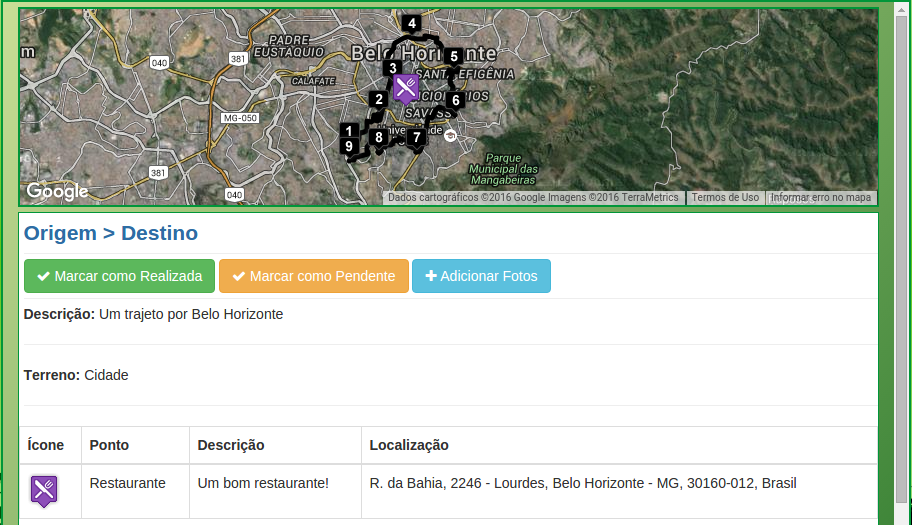
\includegraphics[width=0.8\textwidth]{figuras/marcarRota.png}
	 \vspace{0cm}
	\\\textbf{\footnotesize Fonte: Elaborado pelo autor}
	\label{fig:marcarRota}
\end{figure}

\subsection{Relação de amizade}

O Ciclotour permite relações de amizades entre usuários mediante solicitação. Usuários podem buscar por outros usuários através de seu nome, 
sobrenome e e-mail e enviar solicitação de amizade a este usuário que pode ou não aceitá-la demonstrados na Figura \ref{fig:buscarUsuario} e na 
Figura \ref{fig:solicitacaoAmizade}. A relação de amizade entre usuário permite que os mesmos vejam em seu \textit{feed} as atividades de seus amigos. O 
Ciclotour também possui um contador de amizades que será exibido para outros usuários.

\begin{figure}[!ht]
	\centering	
	\caption[\hspace{0.1cm} Buscar usuários.]
	{Página de busca de usuários e envio de solicitação de amizade}
	  \vspace{-0.4cm}
	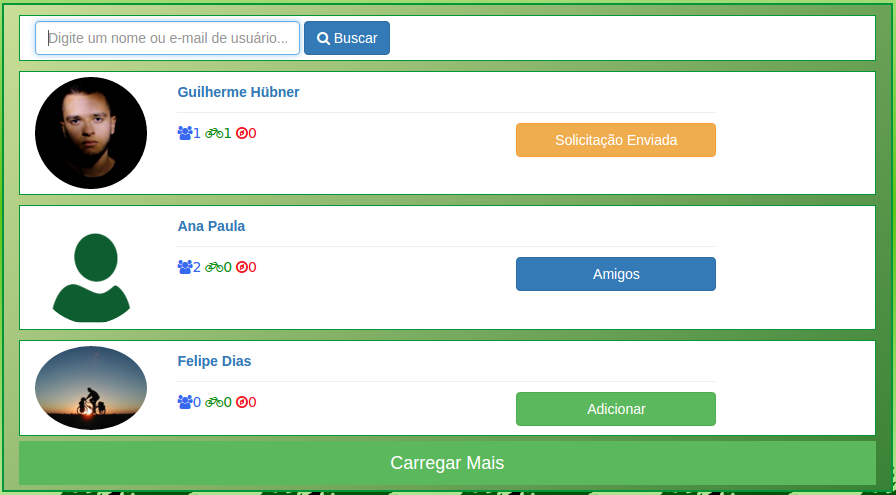
\includegraphics[width=0.8\textwidth]{figuras/buscarUsuario.png}
	 \vspace{0cm}
	\\\textbf{\footnotesize Fonte: Elaborado pelo autor}
	\label{fig:buscarUsuario}
\end{figure}

\begin{figure}[!ht]
	\centering	
	\caption[\hspace{0.1cm} Solicitações de amizade.]
	{Página de onde são exibidas as solicitações de amizade}
	  \vspace{-0.4cm}
	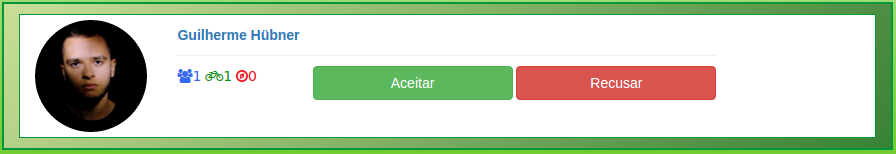
\includegraphics[width=0.8\textwidth]{figuras/solicitacaoAmizade.png}
	 \vspace{0cm}
	\\\textbf{\footnotesize Fonte: Elaborado pelo autor}
	\label{fig:solicitacaoAmizade}
\end{figure}

\subsection{Adicionar fotos em rotas}
Se tratando de uma aplicação voltada ao turismo, é importante que usuários possam compartilhar fotos de suas atividades com outros usuários. Fotos 
podem despertar interesse de outros cicloturistas pela rota, além de ser uma fonte de informação. É muito comum usuários postarem fotos em pontos 
turísticos em outras redes sociais, sendo o Ciclotour uma rede social focada em turismo, este recurso é indispensável.

\section{Conclusão}
Este artigou apresentou a aplicação Ciclotour, uma rede social colaborativa para cicloturistas, cujo objetivo principal é oferecer aos cicloturistas 
um local onde possam interagir com outros cicloturistas, compartilhar e encontrar informações que auxiliem o planejamento de suas atividade, 
oferecendo recursos para atender as necessidades específicas deste meio, percebidas através deste trabalho e que ainda não foram exploradas por 
outras aplicações.

Para trabalhos futuros na aplicação Ciclotour, pretende-se uma melhoria de \textit{design} para atender à requisitos de \textit{User Experience} (UX),
que são fundamentais para sistemas no formato rede social. Além desta melhoria, pretendemos também passar a utilizar a extensão PostGIS no banco de 
dados da aplicação para melhorar o gerenciamento de dados especiais, com esta mudança será possível oferecer ainda mais recursos geográficos na 
aplicação e melhorar os que já são oferecidos.



